\section{Auswertung}
\label{sec:Auswertung}

\subsection{Überprüfung der Bragg Bedingung}

In Tabelle \ref{tab:braggbed} sind die Messwerte zur Überprüfung der braggschen
Bedingung dargestellt. Diese sind in Abbildung \ref{fig:braggbed} als Graph
aufgetragen.
Das Maximum der Kurve liegt bei dem Winkel
\begin{equation}
  \theta_\text{mess} = \SI{28.4}{\degree}.
\end{equation}

Der Sollwert für das Maximum lautet
\begin{equation}
  \theta_\text{soll} = \SI{28}{\degree}.
\end{equation}

\begin{figure}
  \centering
  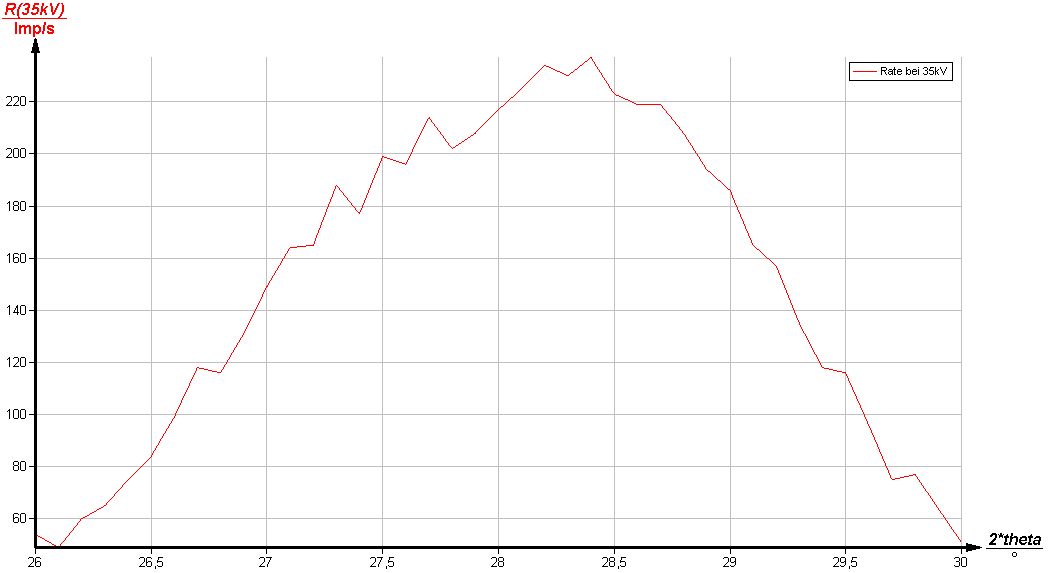
\includegraphics[height=8cm]{Daten/braggbedingung.png}
  \caption{Graph zur Überprüfung der Bragg Bedingung. Es sind die Impulse pro
  Sekunde gegen den Winkel aufgetragen.}
  \label{fig:braggbed}
\end{figure}

\begin{table}[h]
  \centering
  \begin{tabular}{S S}
    \toprule
    {$\theta/\si{\degree}$} & {$Imp/\si{\second}$}\\
    \midrule
    26.0 & 54.0\\
    26.1 & 49.0\\
    26.2 & 60.0\\
    26.3 & 65.0\\
    26.4 & 75.0\\
    26.5 & 84.0\\
    26.6 & 99.0\\
    26.7 & 118.0\\
    26.8 & 116.0\\
    26.9 & 131.0\\
    27.0 & 149.0\\
    27.1 & 164.0\\
    27.2 & 165.0\\
    27.3 & 188.0\\
    27.4 & 177.0\\
    27.5 & 199.0\\
    27.6 & 196.0\\
    27.7 & 214.0\\
    27.8 & 202.0\\
    27.9 & 208.0\\
    28.0 & 217.0\\
    28.1 & 225.0\\
    28.2 & 234.0\\
    28.3 & 230.0\\
    28.4 & 237.0\\
    28.5 & 223.0\\
    28.6 & 219.0\\
    28.7 & 219.0\\
    28.8 & 208.0\\
    28.9 & 194.0\\
    29.0 & 186.0\\
    29.1 & 165.0\\
    29.2 & 157.0\\
    29.3 & 135.0\\
    29.4 & 118.0\\
    29.5 & 116.0\\
    29.6 & 96.0\\
    29.7 & 75.0\\
    29.8 & 77.0\\
    29.9 & 64.0\\
    30.0 & 51.0\\
    \bottomrule
  \end{tabular}
  \caption{Messwerte zur Überprüfung der Bragg Bedingung. Es sind die
  Impulse pro Sekunde gegen den Winkel aufgetragen.}
  \label{tab:braggbed}
\end{table}

\subsection{Das Emissionsspektrum einer CU-Röntgenröhre}

In Tabelle \ref{tab:emission} sind die Messwerte zur Bestimmung des
Emissionsspektrum einer CU-Röntgenröhre abgebildet. Der zugehörige Graph ist
ist in Abbildung \ref{fig:emission} dargestellt.

\begin{figure}
  \centering
  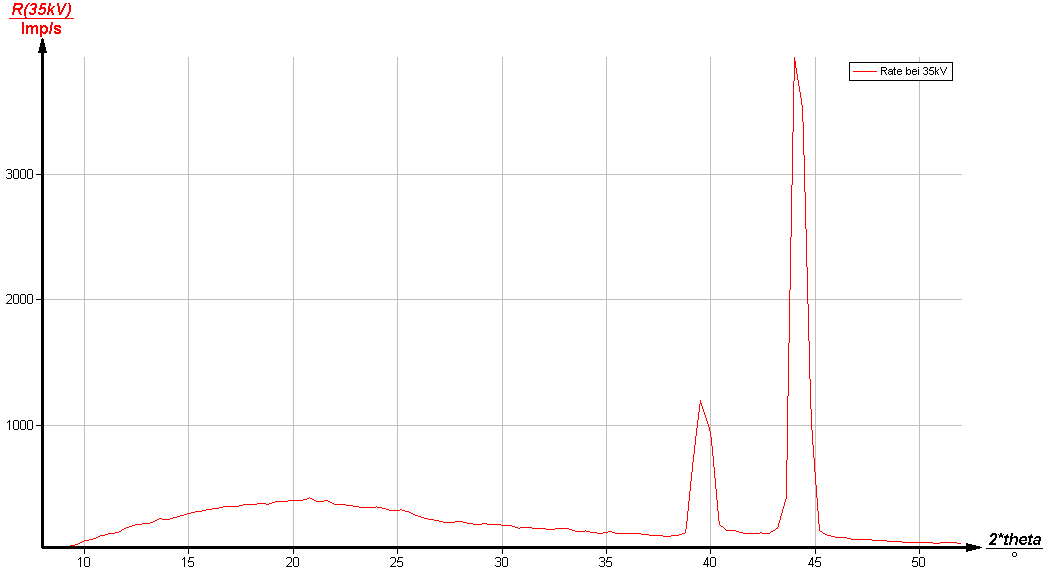
\includegraphics[height=7cm]{Daten/emissionsspektrum.png}
  \caption{Graph des Emissionsspektrums der CU-Röntgenröhre. Es sind die
  Impulse pro Sekunde gegen den Winkel aufgetragen.}
  \label{fig:emission}
\end{figure}

\begin{table}[h]
  \centering
  \begin{tabular}{S S}
    \toprule
    {$\theta/\si{\degree}$} & {$Imp\si{\second}$}\\
    \midrule
    1 & 637.2\\
    \bottomrule
  \end{tabular}
  \caption{Messwerte zur Bestimmung des Emissionsspektrums. Es sind die
  Impulse pro Sekunde gegen den Winkel aufgetragen.}
  \label{tab:emission}
\end{table}

8.8	26,0

\subsection{Absorptionsspektren verschiedener Stoffe}

\subsubsection{Germanium}

Die Messwerte der Germaniumprobe sind in Tabelle \ref{tab:germanium} abgebildet
und als Graph in Abbildung \ref{fig:germanium} dargestellt.
Die gemessene K-Kante befindet sich bei
\begin{equation}
  2\theta_\text{Ge} = \SI{32.4}{\degree}.
\end{equation}
Mit der Bragg'schen Bedingung \eqref{eqn:braggbed} folgt dann für die
Wellenlänge
\begin{equation}
  \lambda_\text{Ge} = \SI{0.1124}{\nano\meter}.
\end{equation}
Mit der Formel
\begin{equation}
  E = \frac{c h}{\lambda}
  \label{eqn:energielambda}
\end{equation}
folgt der Energiewert an der K-Kante für Germanium
\begin{equation}
  E_\text{Ge,mess} = \SI{11.0328}{\kilo\electronvolt}.
\end{equation}

\subsection{Brom}

Die Messwerte der Bromprobe sind in Tabelle \ref{tab:brom} dargestellt und als
Graph in der Abbildung \ref{fig:brom} aufgetragen.
Die gemessene K-Kante befindet sich bei
\begin{equation}
  2\theta_\text{Br} = 25.4 .
\end{equation}
Für die Wellenlänge folgt mit \eqref{eqn:braggbed}
\begin{equation}
  \lambda_\text{Br} = \SI{0.0886}{\nano\meter}.
\end{equation}
Daraus ergibt sich mit Hilfe der Formel \eqref{eqn:energielambda}
der Wert am Energieübergang
\begin{equation}
  E_\text{Br,mess} = \SI{14.0008}{\kilo\electronvolt}.
\end{equation}

\begin{table}[h]
  \centering
  \begin{tabular}{S S}
    \toprule
    {$\theta/\si{\degree}$} & {$Imp/\si{\second}}$}\\
    \midrule
    20.0 & 33.0 \\
    20.2 & 31.0 \\
    20.4 & 33.0 \\
    20.6 & 30.0 \\
    20.8 & 30.0 \\
    21.0 & 29.0 \\
    21.2 & 30.0 \\
    21.4 & 28.0 \\
    21.6 & 29.0 \\
    21.7 & 27.0 \\
    22.0 & 27.0 \\
    22.2 & 26.0 \\
    22.4 & 25.0 \\
    22.6 & 24.0 \\
    22.8 & 25.0 \\
    23.0 & 24.0 \\
    23.2 & 24.0 \\
    23.4 & 23.0 \\
    23.6 & 23.0 \\
    23.8 & 21.0 \\
    24.0 & 23.0 \\
    24.2 & 22.0 \\
    24.4 & 23.0 \\
    24.6 & 22.0 \\
    24.7 & 19.0 \\
    25.0 & 23.0 \\
    25.2 & 28.0 \\
    25.4 & 34.0 \\
    25.6 & 43.0 \\
    25.8 & 47.0 \\
    26.0 & 54.0 \\
    26.2 & 55.0 \\
    26.4 & 53.0 \\
    26.6 & 48.0 \\
    26.8 & 47.0 \\
    27.0 & 46.0 \\
    27.2 & 43.0 \\
    27.4 & 42.0 \\
    27.6 & 41.0 \\
    27.8 & 40.0 \\
    28.0 & 37.0 \\
    28.2 & 34.0 \\
    28.4 & 35.0 \\
    28.6 & 33.0 \\
    28.8 & 32.0 \\
    29.0 & 31.0 \\
    29.2 & 30.0 \\
    29.4 & 29.0 \\
    29.6 & 26.0 \\
    29.8 & 28.0 \\
    30.0 & 27.0 \\
    30.2 & 26.0 \\
    30.4 & 25.0 \\
    30.6 & 23.0 \\
    30.8 & 23.0 \\
    31.0 & 22.0 \\
    31.2 & 22.0 \\
    31.4 & 19.0 \\
    31.6 & 19.0 \\
    31.8 & 21.0 \\
    32.0 & 19.0 \\
    32.2 & 19.0 \\
    32.4 & 16.0 \\
    32.5 & 17.0 \\
    \bottomrule
  \end{tabular}
  \caption{Messwerte der Bromprobe. Es sind die
  Impulse pro Sekunde gegen den Winkel aufgetragen.}
  \label{tab:brom}
\end{table}

\subsection{Bismuth}

In Tabelle \ref{tab:bismuth} sind die Messwerte der Bismuthprobe abgebildet.
Diese sind in Abbildung \ref{fig:bismuth} als Graph aufgetragen.
Die Messung ergibt einen Winkel von
\begin{equation}
  2\theta_\text{Bi} = 22.2 .
\end{equation}
Daraus ergibt sich mit \eqref{eqn:braggbed} die Wellenlänge
\begin{equation}
  \lambda_\text{Bi} = \SI{0.0775}{\nano\meter}.
\end{equation}
Mit \eqref{eqn:energielambda} folgt der Energiewert an der K-Kante von Bismuth
\begin{equation}
  E_\text{Bi,mess} = \SI{15.9879}{\kilo\electronvolt}.
\end{equation}

\subsection{Zirkonium}

Die Messwerte für Zirkonium sind in Tabelle \ref{tab:zirkonium} dargestellt und
in Abbildung \ref{fig:zirkonium} als Graph aufgetragen.

\begin{table}[h]
  \centering
  \begin{tabular}{S S}
    \toprule
    {$\theta/\si{\degree}$} & {$Imp/\si{\second}$}\\
    \midrule
    15.0 & 128.0\\
    15.2 & 134.0\\
    15.4 & 138.0\\
    15.6 & 133.0\\
    15.8 & 131.0\\
    16.0 & 136.0\\
    16.2 & 130.0\\
    16.4 & 132.0\\
    16.6 & 131.0\\
    16.7 & 127.0\\
    17.0 & 132.0\\
    17.2 & 128.0\\
    17.4 & 120.0\\
    17.6 & 121.0\\
    17.7 & 121.0\\
    18.0 & 123.0\\
    18.2 & 120.0\\
    18.4 & 132.0\\
    18.6 & 159.0\\
    18.8 & 190.0\\
    19.0 & 229.0\\
    19.2 & 268.0\\
    19.4 & 283.0\\
    19.6 & 294.0\\
    19.8 & 286.0\\
    20.0 & 286.0\\
    20.2 & 285.0\\
    20.4 & 288.0\\
    20.6 & 276.0\\
    20.8 & 280.0\\
    21.0 & 275.0\\
    21.2 & 279.0\\
    21.4 & 268.0\\
    21.6 & 269.0\\
    21.7 & 260.0\\
    22.0 & 254.0\\
    22.2 & 252.0\\
    22.4 & 242.0\\
    22.6 & 234.0\\
    22.8 & 239.0\\
    23.0 & 223.0\\
    23.2 & 222.0\\
    23.4 & 221.0\\
    23.6 & 213.0\\
    23.8 & 215.0\\
    24.0 & 204.0\\
    24.2 & 205.0\\
    24.4 & 199.0\\
    24.6 & 202.0\\
    24.7 & 197.0\\
    25.0 & 191.0\\
    25.2 & 190.0\\
    25.4 & 178.0\\
    25.6 & 166.0\\
    25.8 & 159.0\\
    26.0 & 155.0\\
    26.2 & 144.0\\
    26.4 & 134.0\\
    26.6 & 130.0\\
    26.8 & 128.0\\
    27.0 & 123.0\\
    \bottomrule
  \end{tabular}
  \caption{Messwerte der Zirkoniumprobe. Es sind die
  Impulse pro Sekunde gegen den Winkel aufgetragen.}
  \label{tab:zirkonium}
\end{table}


Tabelle für copy and paste:
\begin{table}[h]
  \centering
  \begin{tabular}{S S}
    \toprule
    {$k$} & {$U\:/\:\si{\milli\volt}$}\\
    \midrule
    1 & 637.2\\
    3 & 212.4\\
    5 & 127.4\\
    7 & 91.03\\
    9 & 70.8\\
    \bottomrule
  \end{tabular}
  \caption{Amplituden Rechteckspannung.}
  \label{tab:rechtampl}
\end{table}

Literaturwerte:
Atommassen Z
c
e
h
